\section{Antecedentes}
\subsection{Aguas residuales}
La provisión de los servicios de agua potable y de saneamiento es un factor significativo en la salud de la población, ya que evita que estos se expongan a los múltiples agentes patógenos disueltos en las fuentes de consumo disponibles. Por tal motivo, el acceso a estos servicios es crucial para la reducción de la mortalidad y morbilidad entre la población, sobre todo en poblaciones con alto indice de marginalidad \citep{EAM}.\par
Las aguas residuales pueden estar constituidas por diversos constituyentes; dentro de los cuales se destacan los físicos, químicos y biológicos~\citep{crites2000}. Es importante caracterizar los distintos tipos de aguas residuales antes de comenzar con algún proceso para la remoción de contaminantes.\par
\cite{metcalf2003} definen el concepto de aguas residuales como: todas aquellas que, una vez son desechadas por cualquier actividad humana o provenientes de precipitaciones, son vertidas a un sistema de alcantarillado para su posterior tratamiento, o en los casos más comunes, son liberadas directamente en algún cuerpo de agua o sobre una superficie de terreno cualquiera (ver figura \ref{fig:wrts}).\sloppy\par
\begin{figure}[ht]
	\centering
	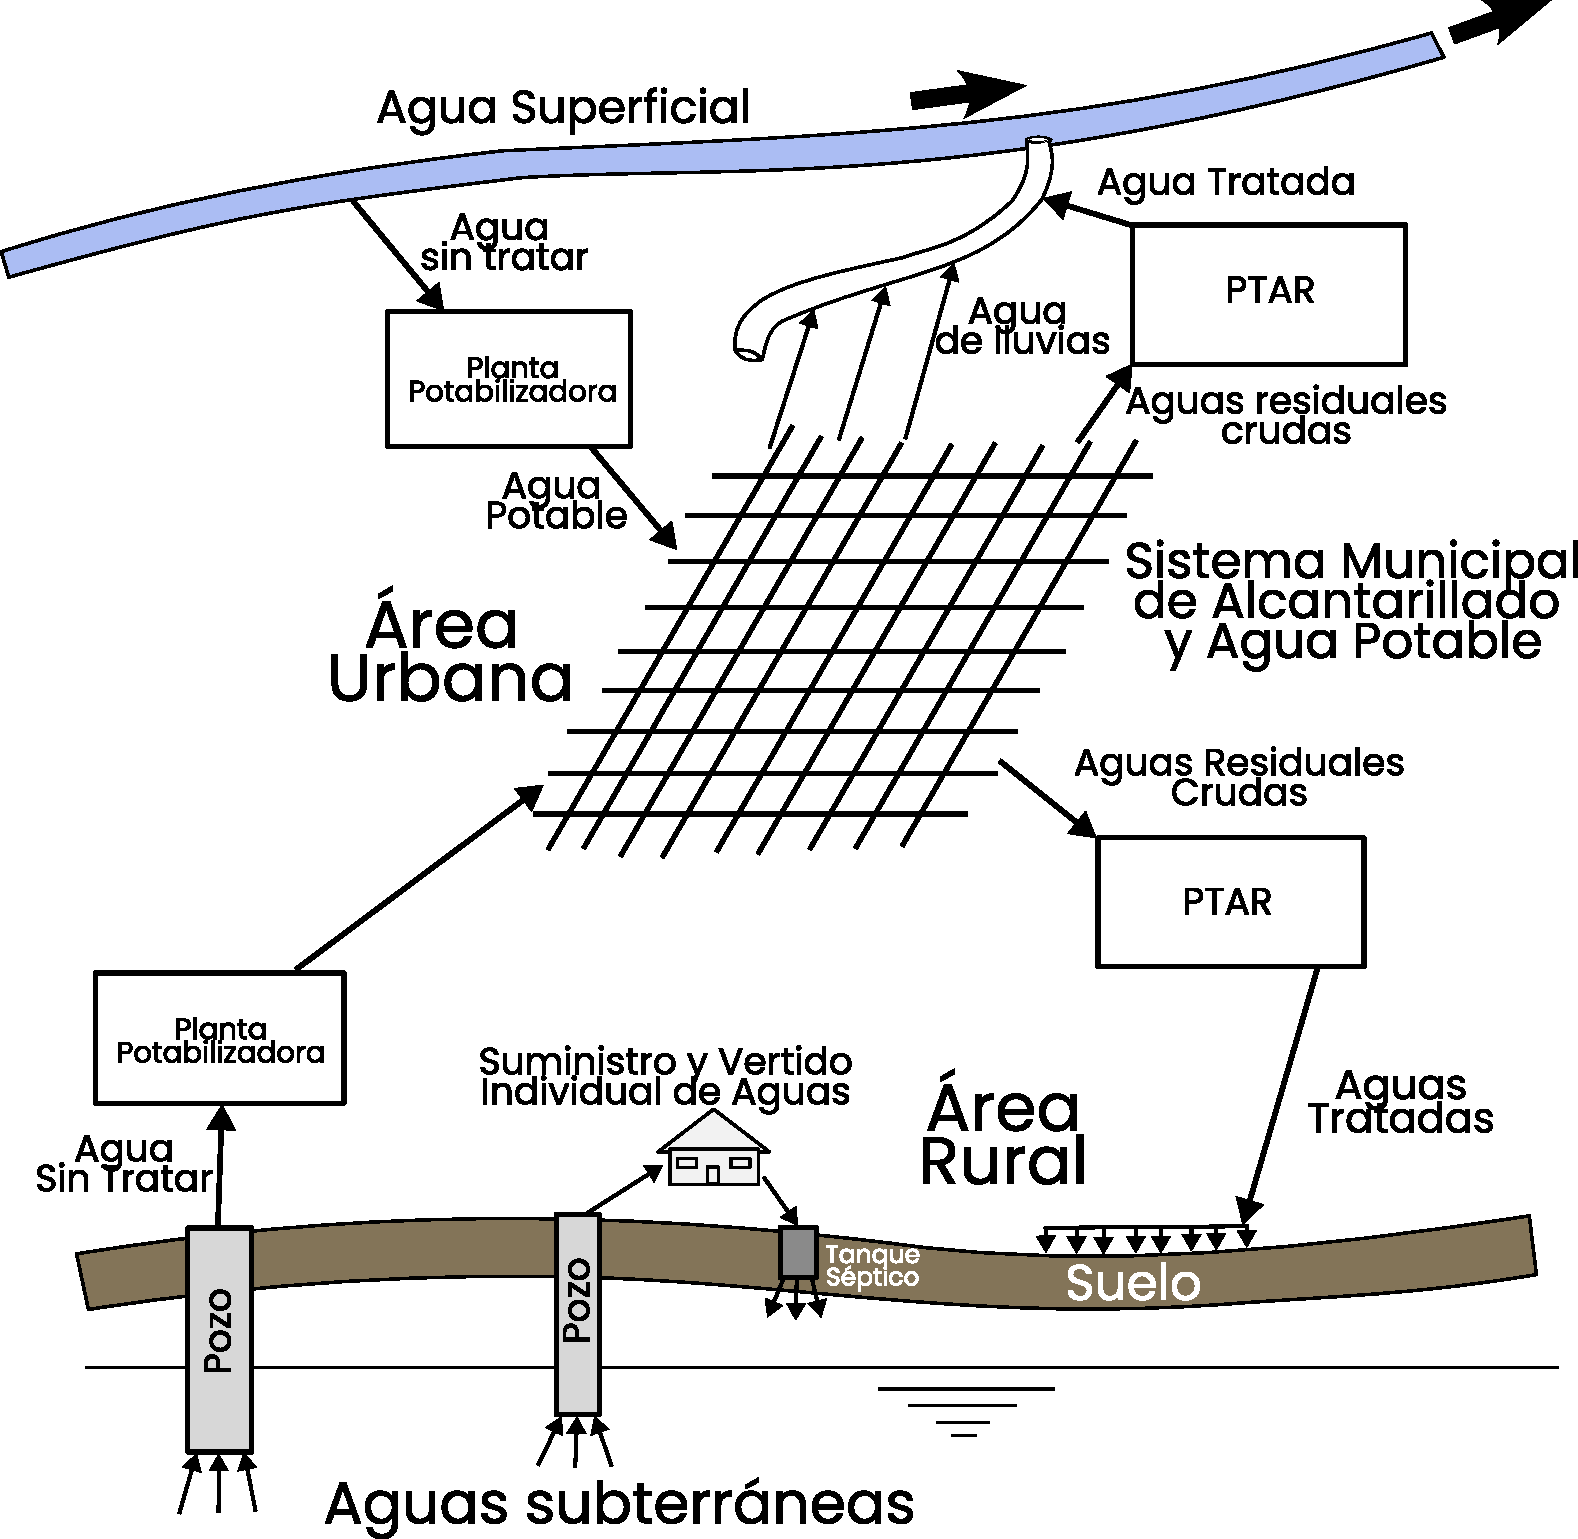
\includegraphics[scale=0.4]{../Images/Water_routes.pdf}
	\\\small{Fuente: Adaptado de \cite{Sperling2007}}
	\caption{Rutas de uso y disposición del agua para actividad humana}\label{fig:wrts}
\end{figure}
Antes de ser vertidas en algún cuerpo de agua o suelo, estas deben ser acondicionadas de acuerdo con los \gls{ECA} establecidos por las normativas presentes en cada país. La misión de estas normativas es mantener una estabilidad en los diferentes ecosistemas, así como el de reducir el número de afecciones a la salud de la población en general~\citep{lazcano2016,martinez1999}. En el caso de México, la \gls{CONAGUA} es la institución encargada de garantizar que se cumplan cada uno de los \acrshort{ECA}s, así como el desarrollar un sistema de puntos de control y monitoreo según las necesidades propias de cada \gls{RHA} \citep{Ortiz2013}. \par
Cabe destacar a este tema que, en la mayoría de países subdesarrollados, la aplicación de estas normativas rara vez se cumplen, resultando en problemas ambientales y de salud graves. La aparición de nuevas industrias locales artesanales y fabricas clandestinas no reguladas provocan un aumento en la cantidad de contaminantes disueltos, entre los cuales, gran parte son metales pesados y/o compuestos de difícil degradación~\cite{metcalf2003}.
Este problema de exacerba cuando no se cuentan con sistemas de tratamiento para las aguas negras generadas por la población, contaminando las distintas fuentes de agua potable de la cuenca en cuestión.\par
A consecuencia de dichas problemáticas, en marzo del 2022, el congreso mexicano logro reformar la \gls{NOM} NOM-001-SEMARNAT-1996, resultando la NOM-001-SEMARNAT-2021 (\emph{ver} Sección \ref{NOM2021}); en tal reforma se actualizan los "límites máximos permisibles de contaminantes en las descargas de aguas residuales en cuerpos receptores propiedad de la nación" \citep{NOM2021}, así como la especificación de cada una de las normas para la cuantificación de los distintos contaminantes a cuantificar y proporcionar sugerencias referentes a la calendarización, métodos de muestreo y contaminantes a analizar.\par
Según sea el caso de uso que recibe el agua es como se clasifica, siendo los principales: aguas residuales domésticas, aguas residuales industriales, aguas pluviales, aguas residuales de origen pecuario y agrícola; y por ultimo las aguas residuales de origen minero-metalúrgico.\par
\subsubsection{Aguas residuales domésticas}
Esta categoría se encuentra conformada por todo aquel flujo de agua proveniente de los hogares\sloppy. Entre los principales constituyentes se incluyen heces y orina de la población; desechos de mascotas, residuos orgánicos producidos por actividades culinarias, desechos de lavandería.\par
\cite{crites2000} las describen como las provenientes de zonas residenciales, comercios, instituciones y espacios recreativos. Algunos de los caudales de descarga típicos se muestran en el cuadro \ref{tab:Qhabituales}. También resulta destacable el mencionar que estos caudales pueden llegar a variar con respecto a la época del año y las condiciones climáticas.\par
\begin{table}[!ht]
	\centering
	\caption{Caudales habituales de agua residual de origen residencial descargada a los sistemas de recolección.}
	\label{tab:Qhabituales}
	\begin{tabular}{llcc}
		\noalign{\hrule height 3pt}
		\multicolumn{2}{c}{}                                    & \multicolumn{2}{c}{Caudal, L/unidad·d} \\ \cline{3-4} 
		\multicolumn{1}{c}{Fuente} & \multicolumn{1}{c}{Unidad} & Intervalo       & Valor habitual       \\ \hline
		Apartamento                &                            &                 &                      \\
		\space~Nivel alto                 & Persona                    & 130--280        & 190                  \\
		\space~Nivel medio                & Persona                    & 190--300        & 250                  \\
		Hotel                      & Huesped                    & 110--210        & 170                  \\
		Residencia individual      &                            &                 &                      \\
		\space~Vivienda nueva             & Persona                    & 170--340        & 170                  \\
		\space~Vivienda vieja             & Persona                    & 110--190        & 150                  \\
		\space~Casa de veraneo            & Persona                    & 100--190        & 150                  \\
		Motel                      &                            &                 &                      \\
		\space~Con cocina                 & Unidad                     & 340--680        & 380                  \\
		\space~Sin cocina                 & Unidad                     & 280--570        & 360                  \\
		Zona de campamento         & Persona                    & 110--190        & 150                  \\ \hline
	\end{tabular}
	\\\small{Fuente:~\cite{crites2000}, cuadro 4.1 p.170.}
\end{table}
Debido a esta naturaleza cambiante, \cite{Fair2008} sugieren que se cuente con planes de muestreo y análisis de las aguas residuales que son vertidas a los sistemas de alcantarillado, esto con la intención de establecer objetivos de control específicos acordes a las condiciones particulares de cada población. Como ejemplo práctico tenemos una comparativa entre Lagos de Moreno, con una población de 172403 habitantes contra una ciudad como Guadalajara, donde la población alcanza la cifra de 1.38 millones de personas~\citep{INEGIJAL}. Mientras que en Lagos de Moreno apenas y se alcanza una décima parte de la población de Guadalajara, la cantidad de industrias locales no llega a alcanzar un punto de comparación, tanto en el rubro(siendo en Lagos el principal rubro el de alimentación, producción agropecuaria y en menor medida la manufactura de piezas automotrices; mientras que en el caso de Guadalajara se destaca la producción automotriz, la manufactura de componentes eléctrico-electrónicos, cadena de suministro, y en ultimo lugar la producción de alimentos y bebidas), como en la carga laboral~\citep{Eunice2022,Lagosjal}.
\begin{figure}[H]
	\centering
	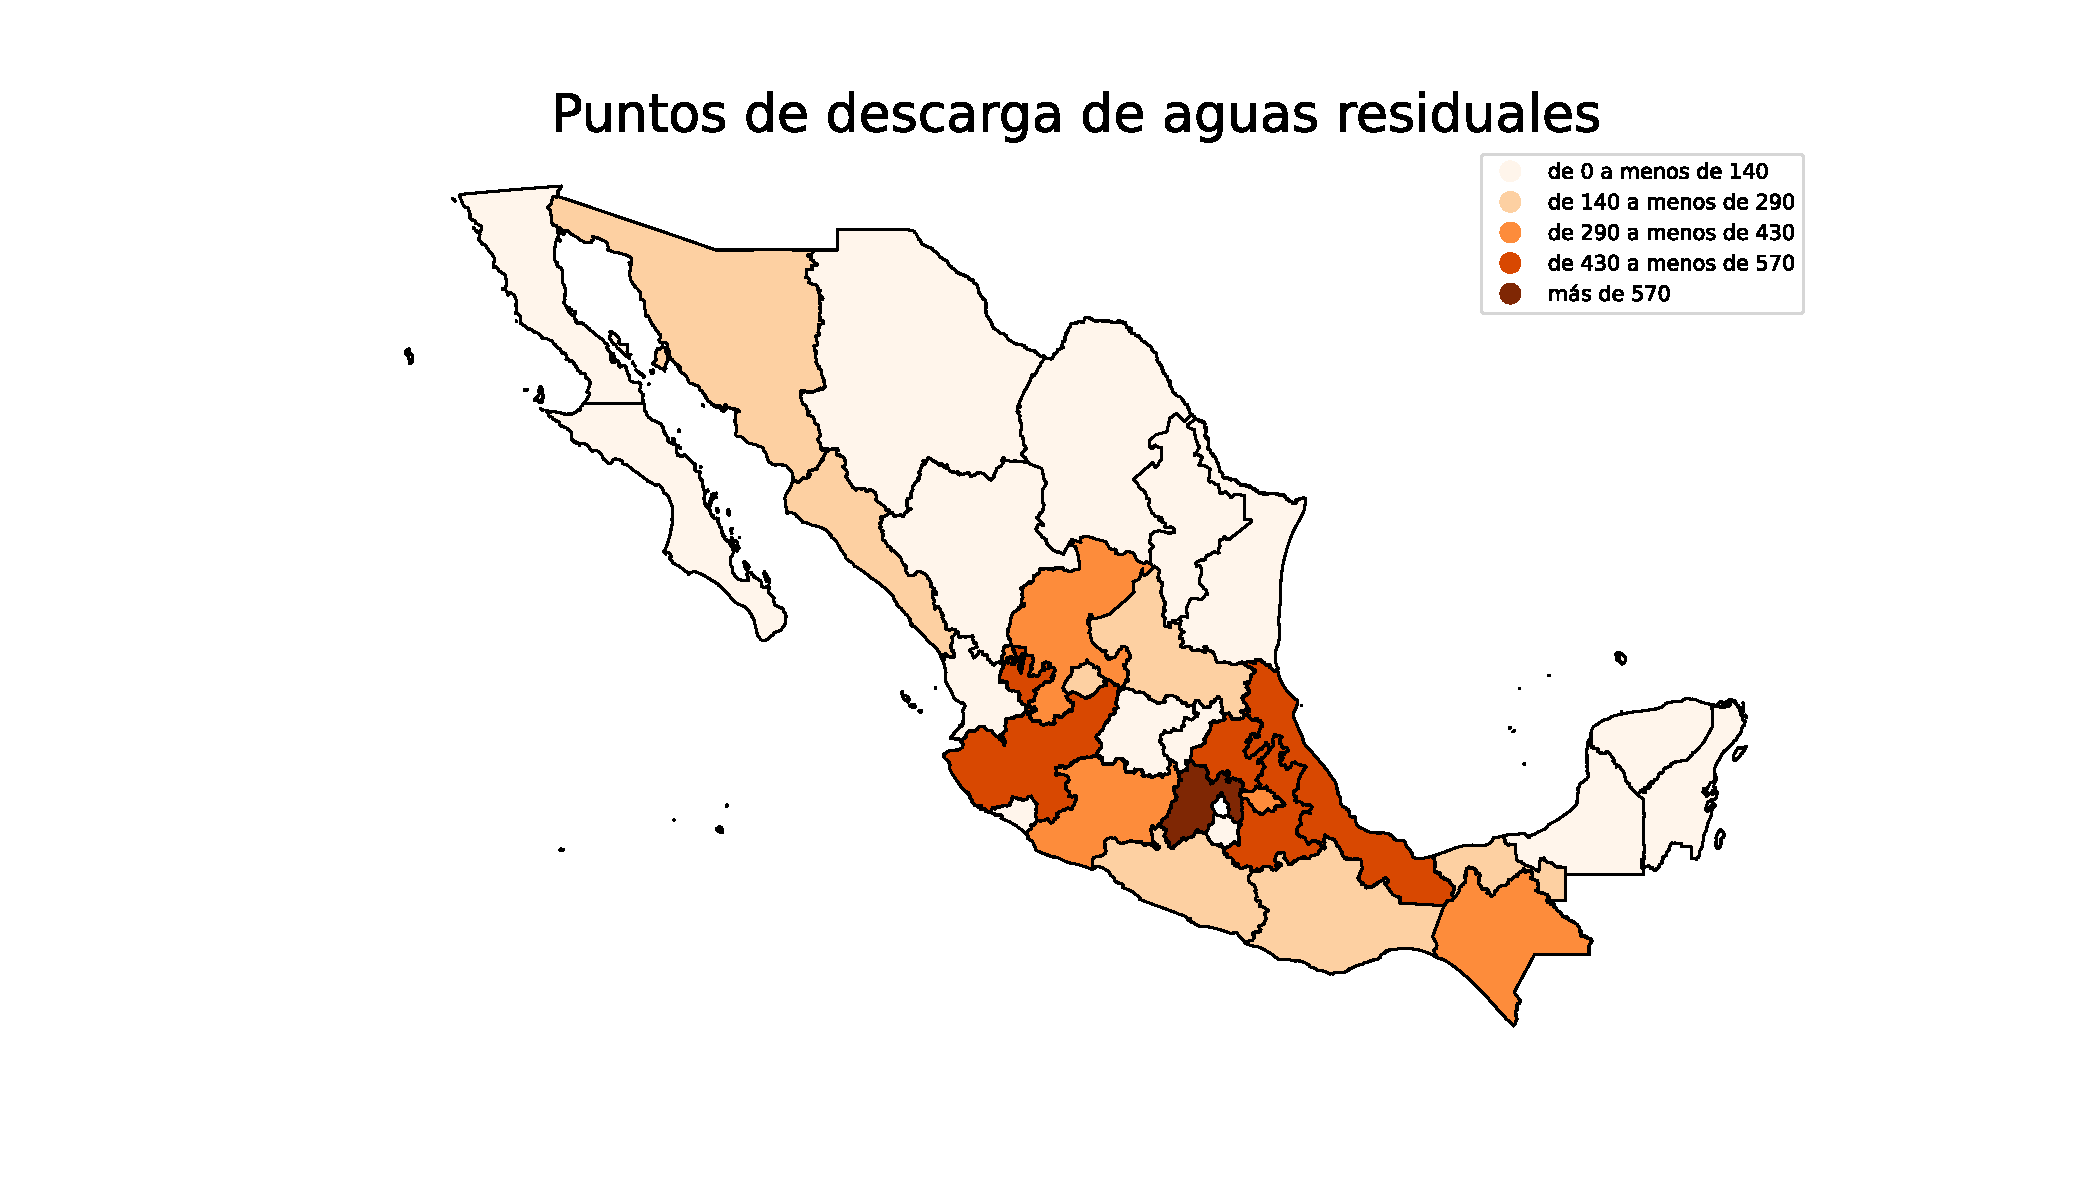
\includegraphics[scale=0.45]{../Images/DescargasTotales.pdf}
	\\\small{Fuente: \cite{Censo2021}}
	\caption{Número total de puntos de descargas de aguas residuales a cuerpos receptores, suelo, barranca o grieta sin algún tipo de tratamiento previo.}\label{puntosdesecho}
\end{figure}
\subsubsection{Aguas residuales municipales}
Este tipo de aguas provienen de la mezcla de los \glspl{efluente} domésticos, de las distintas actividades realizadas en las áreas urbanas (oficinas, tiendas, centros comerciales, restaurantes, actividades recreativas, etc.) y de las pequeñas industrias locales, las cuales aumentan la cantidad de contaminantes y sustancias indeseadas que dificultan su tratamiento mediante sistemas convencionales aplicados a pequeñas comunidades~\citep{lazcano2016}.\par
En 2020 la cobertura de alcantarillado a red pública o fosa séptica fue de 93.8\%. También se tiene la cobertura de acceso a los servicios de alcantarillado y saneamiento básico, que considera la población con drenaje conectado a la red pública, a fosa séptica o con desagüe a suelo, barranca, grieta, río, lago o mar (ver figura \ref{puntosdesecho}).
\begin{figure}[H]
	\centering
	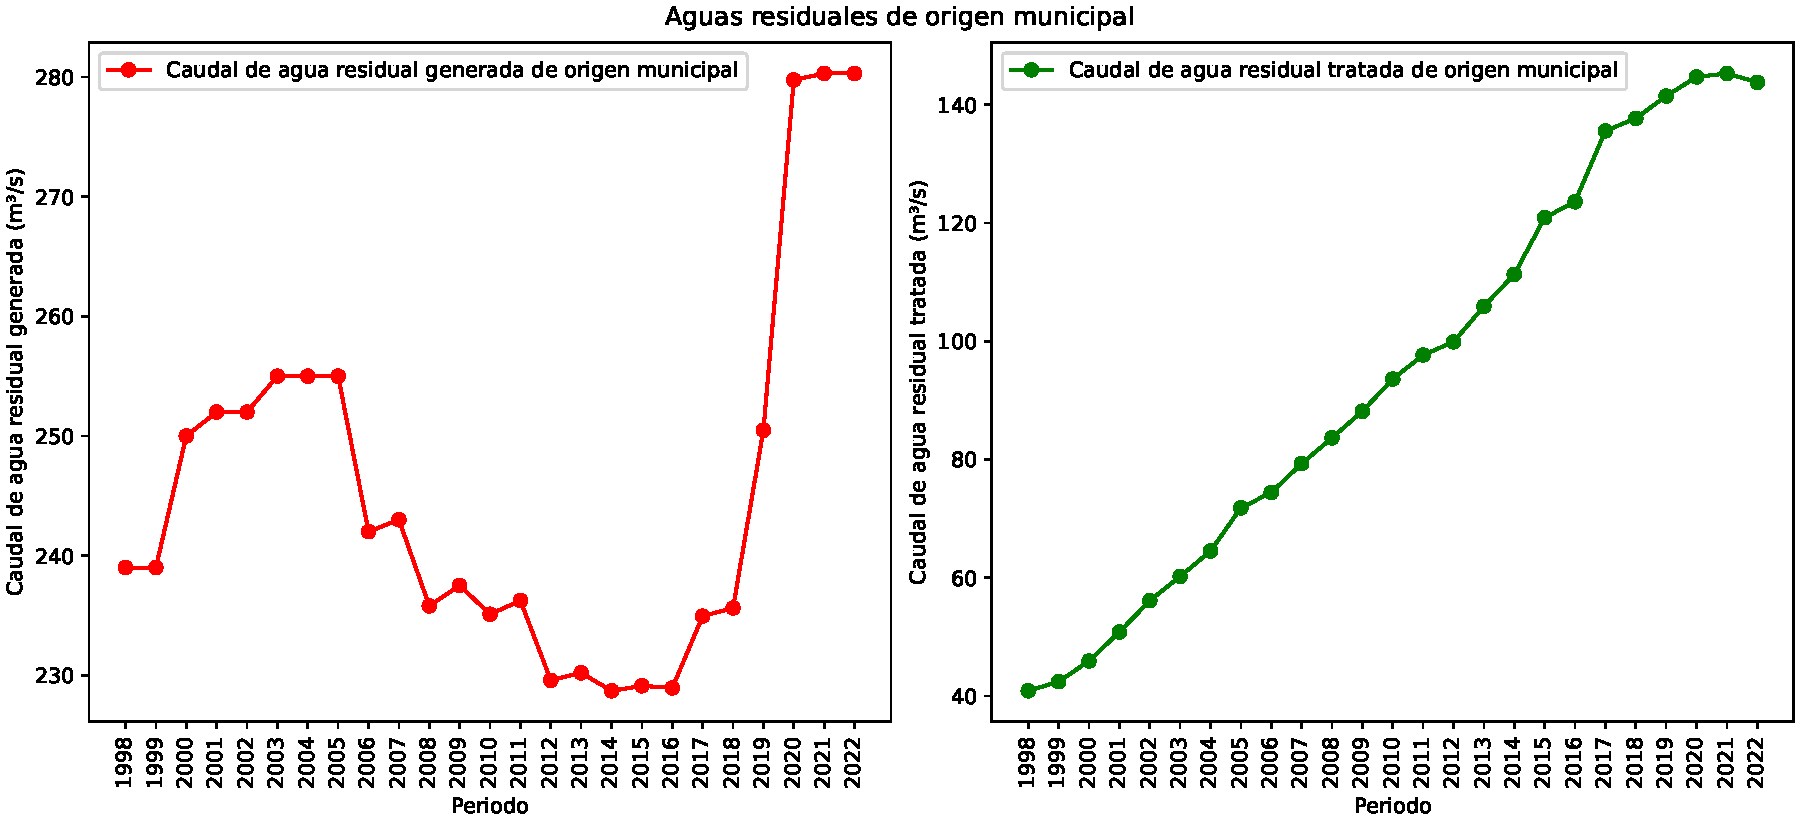
\includegraphics[scale=0.45]{../Images/AR_municipal_svg-tex.pdf}
	\\\small{Fuente: \cite{ODS23}}
	\caption{Caudal de aguas residuales de tipo municipal generadas comparado al caudal de aguas que reciben algún tratamiento}\label{aguamun}
\end{figure}
Tomando en cuenta datos estadísticos del \acrshort{INEGI}, las 2462 plantas en operación a lo largo del país, trataron 141.5 m\textsuperscript{3}/s, es decir el 65.7\% de los 215.3 m\textsuperscript{3}/s recolectados a través de los sistemas de alcantarillado. Para el año 2020, las 2786 plantas en operación trataron 144.7 m\textsuperscript{3}/s, es decir el 67.2\% de los 215.4 m\textsuperscript{3}/s (ver figura \ref{aguamun}) en los sistemas de alcantarillado \citep{EAM}.
\subsubsection{Aguas residuales industriales}
Este tipo de aguas provienen de las grandes industrias, a diferencia de las anteriores, estas se caracterizan por estar fuera de las zonas pobladas y debido a su alto contenido en partículas recalcitrantes, estas deben de recibir un tratamiento previo a ser vertidas a los sistemas de alcantarillado público. generalmente cuentan con un número elevado de metales pesados, pH extremo, altos niveles de materia orgánica, solventes y sustancias tóxicas~\citep{lazcano2016}.\par
La cantidad y composición de las diferentes sustancias contaminantes se ven relacionadas al tipo de proceso que se realiza, así como a la disposición que cada industria toma respecto al tratamiento de sus residuos \citep{Hanchang2009}.\par
\begin{table}[H]
	\begin{adjustbox}{max width=\textwidth}
	\begin{threeparttable}[b]
		\centering
		\caption{Variación entre el flujo y las características de ciertos residuos industriales representativos}
		\label{tab:indwst}
		\begin{small}
			\begin{tabular}{llllllllllll}
				\hline
				\multirow{2}{*}{\begin{tabular}[c]{@{}l@{}}Industria generadora\\del residuo\end{tabular}} & \multicolumn{3}{l}{\begin{tabular}[c]{@{}l@{}}Flujo en gal/unidad\\de producción\end{tabular}} & \multirow{2}{*}{} & \multicolumn{3}{l}{\begin{tabular}[c]{@{}l@{}}DBO5 en lb/unidad\\de producción\end{tabular}} & \multirow{2}{*}{} & \multicolumn{3}{l}{\begin{tabular}[c]{@{}l@{}}Solidos suspendidos en\\lb/unidad de producción\end{tabular}} \\ \cline{2-4} \cline{6-8} \cline{10-12} 
				& 10\%                           & 50\%                           & 90\%                           &                   & 10\%                           & 50\%                          & 90\%                          &                   & 10\%                                & 50\%                               & 90\%                               \\ \hline
				Pulpa y papel$^\dagger$                                     & 11000                          & 43000                          & 74000                          & \multirow{5}{*}{} & 17                             & 58                            & 110                           & \multirow{5}{*}{} & 26                                  & 105                                & 400                                \\
				Cartón$^\dagger$                                            & 7500                           & 11000                          & 27500                          &                   & 10                             & 28                            & 46                            &                   & 25                                  & 48                                 & 66                                 \\
				Rastro$^\ddagger$                                            & 165                            & 800                            & 4300                           &                   & 3.8                            & 13                            & 44                            &                   & 3                                   & 9.8                                & 31                                 \\
				Cervecería$^\S$                                        & 130                            & 370                            & 600                            &                   & 0.8                            & 2                             & 44                            &                   & 0.25                                & 1.2                                & 2.45                               \\
				Curtido de pieles$^\P$                                 & 4.2                            & 9                              & 13.6                           &                   & 575$^{\dagger\dagger}$                            & 975                           & 1400                          &                   & 600$^{\dagger\dagger}$                                 & 1900                               & 3200                               \\ \hline
			\end{tabular}
		\end{small}
		\begin{tablenotes}
			\item{\footnotesize{$\dagger$ Ton de papel producido; 1 Ton=907 Kg}}
			\item{\footnotesize{$\ddagger$ 1000 lb de peso sin sacrificar}}
			\item{\footnotesize{$\S$ Barril de cerveza; 1 barril=0.164 m\textsuperscript{3}}}
			\item{\footnotesize{$\P$ Libras de pieles; sulfuros expresados como S varían de 260 mg/L (10\%) a 1230 mg/L (90\%)}}
			\item{\footnotesize{$\dagger\dagger$ En mg/L}}
		\end{tablenotes}
	\end{threeparttable}}
	\end{adjustbox}
	\centering
	\small{Fuente: \cite{Eckenfelder2000}}
\end{table}
Si la zona de estudio cuenta con una amplia cantidad de industrias que descargan sus residuos directamente al sistema de alcantarillado público, resulta aún más importante la planeación y diseño de la planta de tratamiento, puesto que la carga de contaminantes, junto con los caudales de operación se ven alterados \citep{Sperling2007}.\par
\begin{figure}[H]
	\centering
	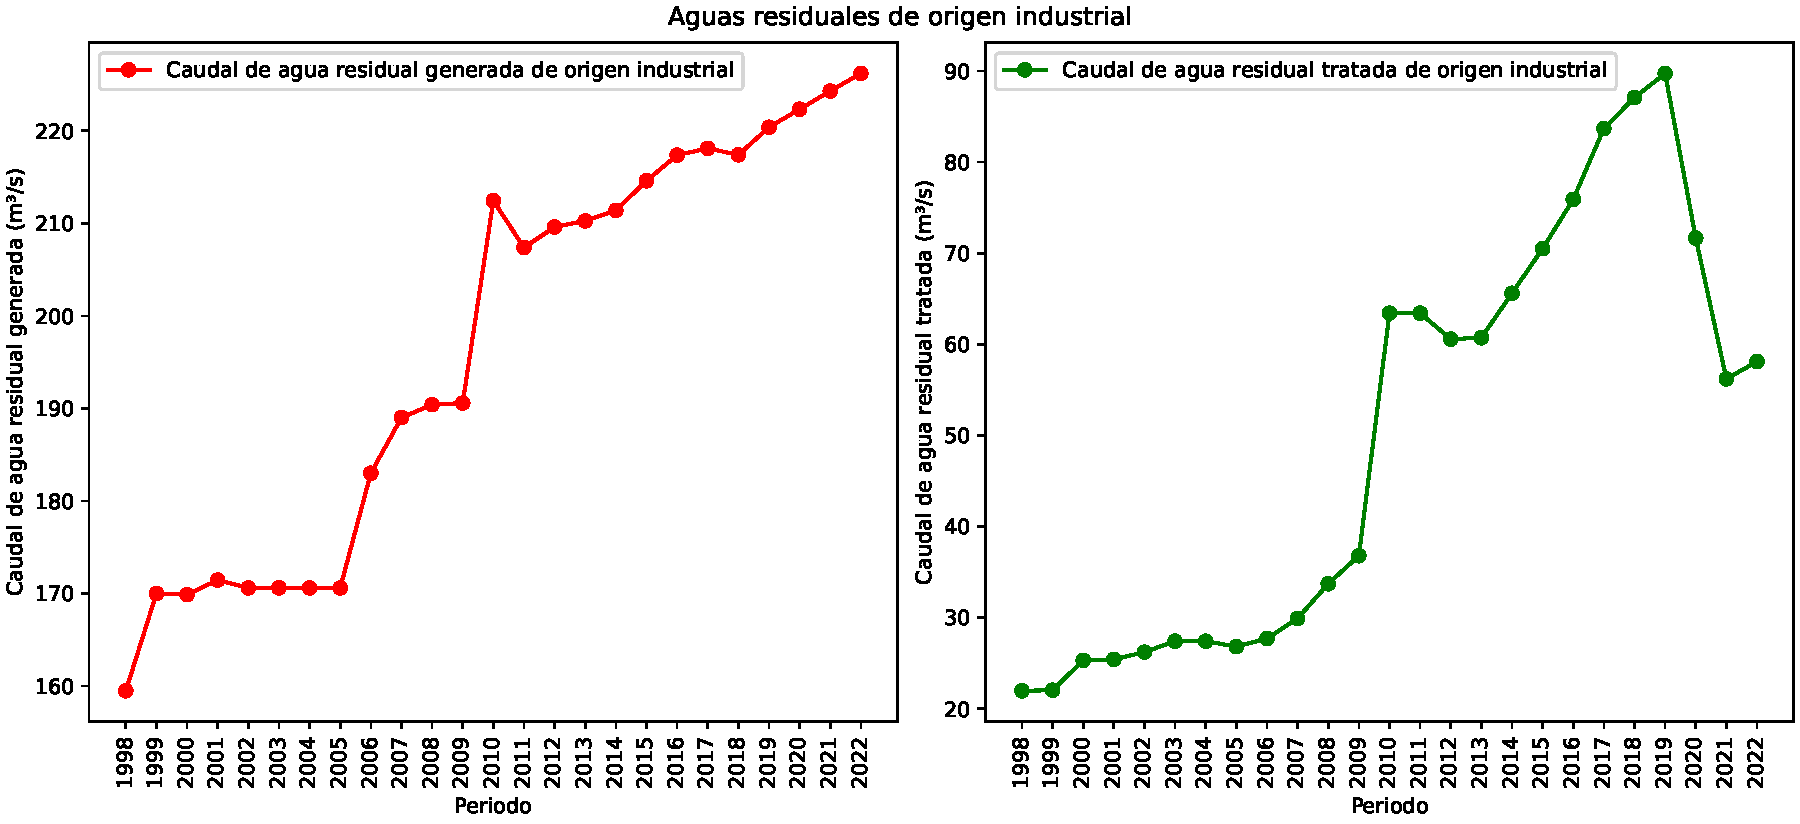
\includegraphics[scale=0.45]{../Images/AR_industrial.pdf}
	\\\small{Fuente: \cite{ODS23}}
	\caption{Caudal de aguas residuales de tipo industrial generadas comparado al caudal de aguas que reciben algún tratamiento}\label{aguaind}
\end{figure}
Se cuentan con datos que en el año 2019, la industria trató 89.77 m\textsuperscript{3}/s de aguas residuales, con un total de 3531 plantas en operación, mientras que, en el año 2020 el caudal tratado y el número de plantas disminuyeron a 71.67 m\textsuperscript{3}/s y 3307 respectivamente \citep{EAM}.\par

\subsubsection{Aguas residuales agropecuarias o agroindustriales}
Son todos aquellos flujos de agua provenientes de cualquier actividad agrícola y pecuaria. Se encuentran constituidas por una gran cantidad de materia orgánica proveniente del estiércol y purines de los animales, residuos derivados del uso de pesticidas, fertilizantes y residuos farmacéuticos de uso veterinario~\citep{lazcano2016}.\par
\cite{zambrano2009} destacan que este tipo de aguas residuales difieren según la forma en la que se tiene el ganado, la forma en que son eliminados los residuos y el estado en el que se encuentran estos. Al tener al ganado disperso en libre pastoreo, el riesgo de contaminación aumenta, ya que se depende de las condiciones hidrológicas del terreno para la dispersión de las excretas del ganado, contaminando así de manera difusa la cuenca en donde se encuentra la explotación y las cuencas aledañas por medio del arrastre de los contaminantes a través de escorrentías superficiales durante el temporal de lluvias.
El tipo de residuos generados por las actividades pecuarias resultan similares a los del tipo doméstico, diferenciándose de los últimos en el volumen de agua con el que son desechados; generando como resultado directo la elevada carga de materia orgánica y sólidos en suspensión.\par
\begin{table}[H]
	\begin{threeparttable}[b]
		\centering
		\caption{Comparación de valores obtenidos en campo con los límites máximos permisibles en sistemas pecuarios}
		\label{tab:Aguaagro}
		\begin{tabular}{lcc}
			\noalign{\hrule height 3pt}
			Indicador                      & Valores \emph{in-situ} & Límites máximos permisibles\tnote{1} \\
			\hline
			pH                             & 7.2             & 6--9                    \\
			DBO\textsubscript{5} (mg/L)                    & 335             & --$^{*}$                          \\
			DQO (mg/L)                     & 733             & 150                          \\
			Conductividad eléctrica (S/cm) & 1100            & --$^{*}$                        \\
			Sólidos Suspendos (mg/L)     & 10.5            & 60                           \\
			Nitrógeno total (mg/L)         & 42.9            & 25                           \\
			Fósforo total (mg/L)           & 9.17            & 15  \\ \hline      
		\end{tabular}
		\begin{tablenotes}
			\item [1] \footnotesize{Según datos de la NOM-001-SEMARNAT-2021}
			\item[*] \footnotesize{Datos no contemplados dentro de la NOM-001-SEMARNAT-2021}
		\end{tablenotes}
	\end{threeparttable}
		\centering
		\\\small{Fuente: Adaptado de \cite{Perez2005}}
\end{table}
En relación al uso agrícola del agua, se tiene como sector prioritario por su impacto en el desarrollo económico y de salubridad, ya que gran parte de la alimentación mundial depende del riego \citep{EAM}. Gracias a la alta demanda en la producción agrícola es que el uso de agroquímicos y pesticidas ha aumentado a un ritmo alarmante, contaminando gran parte de las fuentes de agua potable con residuos potencialmente carcinógenos.
\subsubsection{Aguas residuales de orígen minero-metalúrgico}
Los efluentes provenientes de la actividad minera son considerados los más tóxicos debido a su alto contenido en metales pesados como el plomo, mercurio, cadmio y zinc; ademas de metaloides antimonio y el arsénico. En países donde la mayor parte de las regulaciones son ignoradas o no son tan estrictas, la cantidad de estos elementos tóxicos supera con creces los límites máximos permitidos, dificultando aún más el tratamiento por medios convencionales. Debido a su alto número en compuestos abióticos, es necesario que este tipo de afluentes reciban un tratamiento anterior a la entrada de cualquier sistema de tratamiento biológico~\citep{lazcano2016}.
La presencia de metales pesados en concentraciones elevadas puede provocar la acidificación del agua y generar condiciones adversas para la vida acuática. Además, la liberación de sustancias tóxicas puede tener impactos a largo plazo en los ecosistemas acuáticos y terrestres, afectando la biodiversidad y la calidad del suelo \citep{Kamberovic2012}.\par
El tratamiento de aguas residuales minero-metalúrgicas a menudo requiere enfoques especializados. Las tecnologías convencionales de tratamiento de aguas residuales pueden ser insuficientes debido a la complejidad de los contaminantes presentes. Los métodos como la precipitación química, la coagulación-floculación, la adsorción y la electrocoagulación se utilizan para la remoción eficiente de metales y compuestos tóxicos\sloppy~\citep{wu2017,Kamberovic2012}. La investigación continua en tecnologías emergentes, como la fitoextracción y la biorremediación, busca abordar de manera sostenible la problemática de las aguas residuales minero-metalúrgicas. Estas técnicas involucran el uso de plantas o microorganismos para absorber o degradar contaminantes, ofreciendo enfoques más ecológicos para la rehabilitación de sitios mineros contaminados~\citep{Sulimova2016}.
\subsubsection{Aguas pluviales}
Aquellas aguas provenientes de las precipitaciones que terminan en las alcantarillas logran disminuir la carga orgánica que hay en el desagüe, sin embargo, el cambio en las concentraciones produce variaciones en las características fisicoquímicas del agua~\citep{lazcano2016}.\par
Para abordar estos problemas, se han implementado diversas estrategias de gestión de aguas pluviales, como la construcción de infraestructuras de retención de agua, la implementación de prácticas de diseño urbano sostenible y la promoción de sistemas de alcantarillado separados para aguas pluviales y aguas residuales. Estas medidas buscan minimizar la entrada de aguas pluviales en los sistemas de tratamiento de aguas residuales y reducir los impactos adversos asociados~\citep{EPA}.\par
\begin{figure}[H]
	\centering
	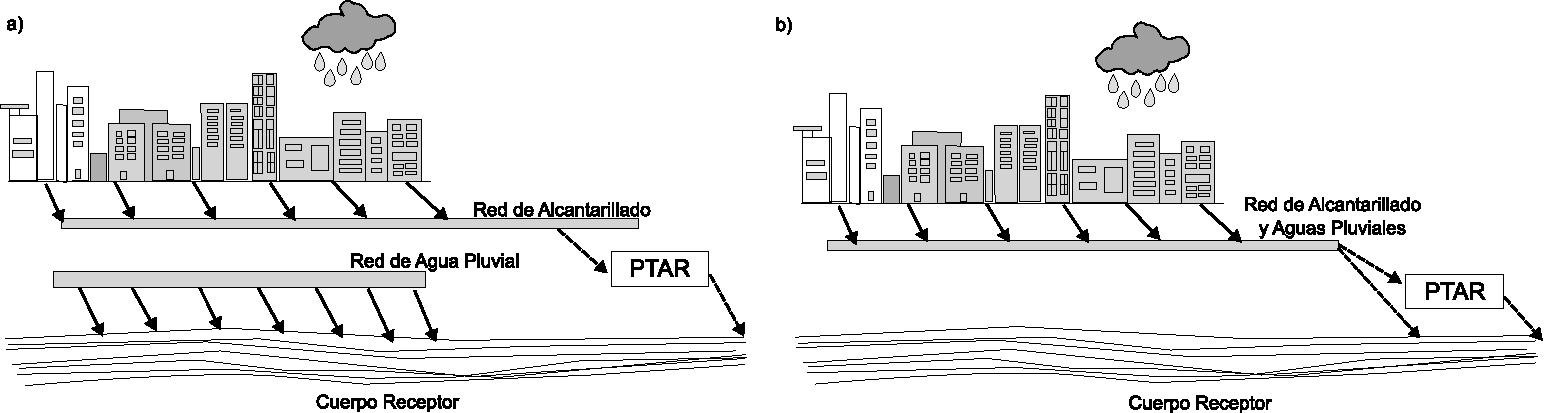
\includegraphics[scale=0.45]{../Images/Sewage_systems.pdf}
	\\\small{Fuente: \cite{Sperling2007}}
	\caption{Tipos principales de sistemas de recolección de aguas residuales municipales.}\label{fig:swgstm}
\end{figure}
En este punto es necesario mencionar la importancia que tiene el diseño de los sistemas de alcantarillado publico presentes en las ciudades, destacando los sistemas separados en contra de los sistemas combinados durante los temporales de lluvia, ya que estos evitan la sobresaturación de las plantas municipales en caso de tormentas torrenciales, reduciendo daños potenciales que afecten al funcionamiento de todo el sistema de tratamiento \citep{Sperling2007}.\par
La creación de sistemas de alcantarillado separados para aguas pluviales y aguas residuales evita la sobrecarga de los sistemas de tratamiento de aguas residuales durante eventos de lluvia intensa (ver figura \ref{fig:swgstm}). Esto permite que las aguas pluviales fluyan directamente hacia cuerpos de agua locales sin pasar por plantas de tratamiento~\citep{WEF}.\par
Es importante señalar que la implementación de estas medidas puede variar según la ubicación geográfica y las características específicas de cada área. Las autoridades locales, agencias ambientales y organizaciones especializadas suelen ser fuentes valiosas de información sobre regulaciones y mejores prácticas adaptadas a contextos particulares.\par
\subsection{Características de las aguas residuales}
Gran parte de los sistemas de desagüe domésticos se encuentran compuestos por un 99.9\% de agua, dejando un 0.1\% compuesto principalmente por compuestos orgánicos e inorgánicos, sólidos suspendidos y disueltos junto con microorganismos. Debido a la presencia de estos polulantes es que se requiere un tratamiento adecuado a fin de salvaguardar la ecología de los distintos ecosistemas, así como el reducir el número de muertes causadas por infecciones gastrointestinales causadas por el uso de aguas servidas como agua de riego en hortalizas (sobre todo en hortalizas que se desarrollan a nivel de suelo) \citep{Sperling2007}.\par
Gran parte de estos contaminantes le otorgan características propias al agua residual, entre estas se destacan:
	\begin{itemize}
		\item Turbidez, causada por la presencia de sólidos suspendidos 
		\item Olor, principalmente por la presencia de ácido sulfhídrico, compuestos orgánicos volátiles y metano en caso de anaerobiosis.
		\item Color, principalmente colores verdes por la presencia de microalgas y microorganismos fotosintéticos; y negro, debido a la acumulación de ácido sulfhídrico en las tuberías de desagüe y la ausencia de oxígeno.
	\end{itemize}
Estas características físicas son esenciales para la evaluación y el diseño de sistemas de tratamiento de aguas residuales, asegurando que estos sistemas sean eficientes y capaces de manejar la diversidad de aguas residuales que se encuentran en diversas fuentes.\par
De estos componentes generales se puede subdividir aún más en diferentes características, denotando como principales las que se enunciarán a continuación.\par
\subsection{Características Físicas}
Las características físicas de las aguas residuales se refieren a las propiedades físicas cuantitativas y cualitativas del agua que ha sido utilizada en diversas actividades humanas antes de su descarga al medio ambiente o su tratamiento. Estas características proporcionan información importante sobre la calidad y la naturaleza del agua residual~\citep{metcalf2003}.\par
Algunas de las características que se mencionaran enseguida se ven influenciadas por el diseño y las características de los sistemas de recolección y transporte de las aguas servidas, siendo importante en estos la implementación de conceptos de hidráulica, materiales, ingeniería civil, planeación urbanística, etc.\par
\begin{figure}[H]
	\centering
	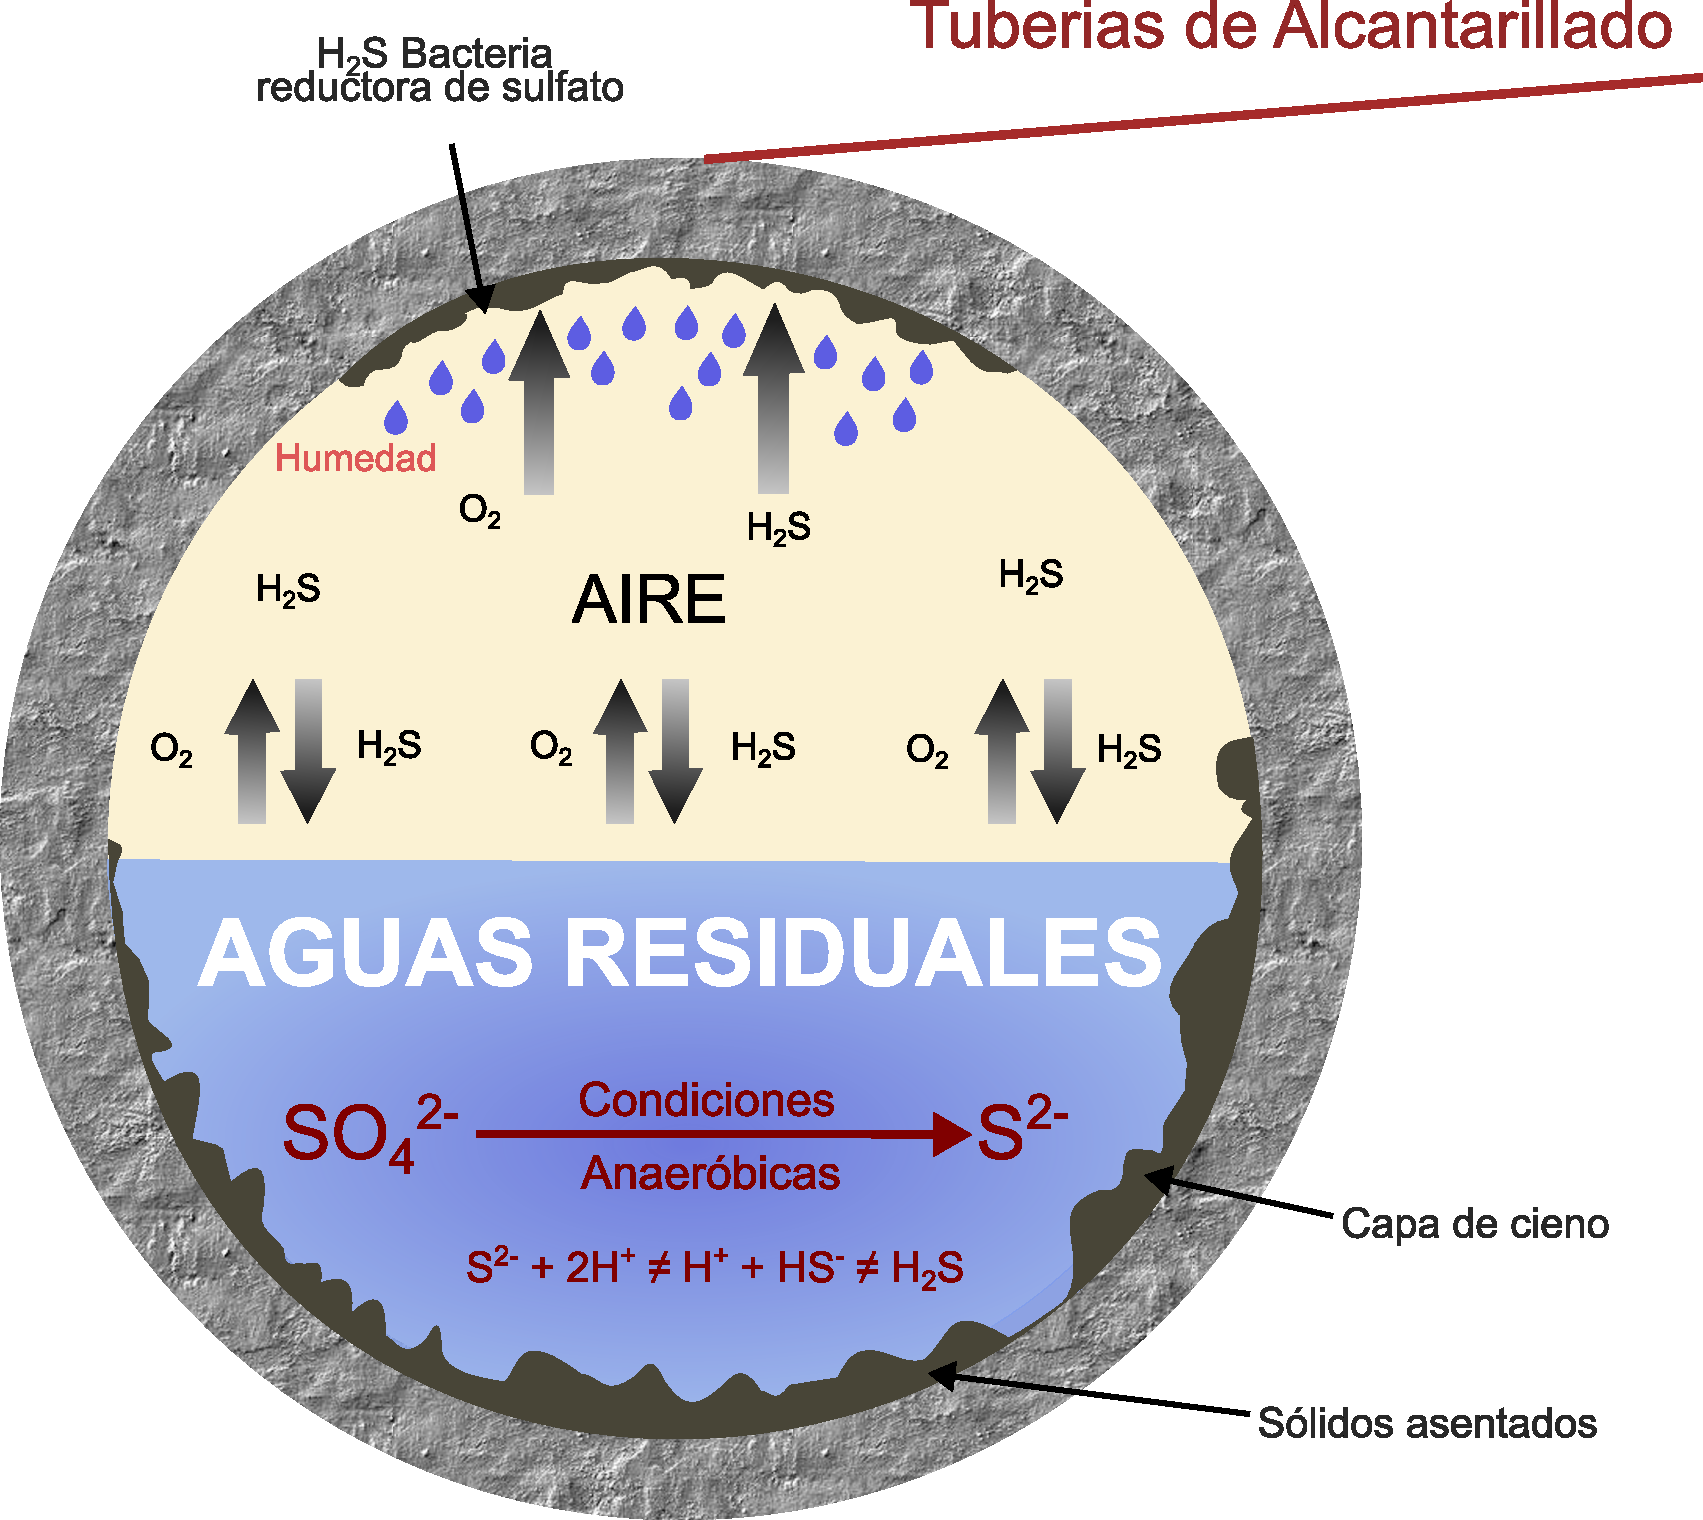
\includegraphics[scale=0.25]{../Images/Tuberia.pdf}
	\\\small{Fuente: \cite{MSASA}}
	\caption{Vista transversal de una tubería de alcantarillado, donde se aprecia de manera general las condiciones de corrosión y generación de gases a las que es sometida habitualmente}\label{fig:tba}
\end{figure}
Un ejemplo práctico de esto es el caudal de las aguas residuales, que es la cantidad de agua que fluye en un período específico, es una característica clave que determina la capacidad de carga de los sistemas de tratamiento. Este parámetro, medido en unidades como litros por segundo o metros cúbicos por segundo, es fundamental para dimensionar infraestructuras y garantizar un manejo efectivo de las aguas residuales en sistemas urbanos e industriales~\citep{crites2000}. Al ser un sistema dinámico, se infiere que las condiciones dentro de los sistemas de alcantarillado pueden pasar de un extremo a otro en cuestión de segundos (sobre todo teniendo en cuenta que en los sistemas centralizados de alcantarillado suelen mezclarse los distintos tipos de aguas residuales ya mencionados anteriormente en el presente texto), por tal motivo las tuberías deben resistir condiciones de altas presiones, taponamientos por acumulación de residuos, generación de gases tóxicos, vibraciones y desplazamientos del terreno, entre un largo etcétera de factores ambientales (ver figura \ref{fig:tba}).
\subsubsection{Sólidos}
Uno de los principales componentes físicos presentes en las aguas residuales son los materiales sólidos dispersos por todo el afluente. El tamaño de estas partículas puede variar desde cabellos hasta materiales coloidales~\citep{metcalf2003}. 
La clasificación de los distintos sólidos se realiza tomando en cuenta el estado y la naturaleza de los componentes de la muestra a analizar, además, varios de estos se pueden agrupar en varios subgrupos en común según la fracción en la que se encuentran y el método por el cual se pueden determinar (ver figura~\ref{fig:solrelcn}); entre los que se identifican:
\begin{figure}[H]
	\centering
	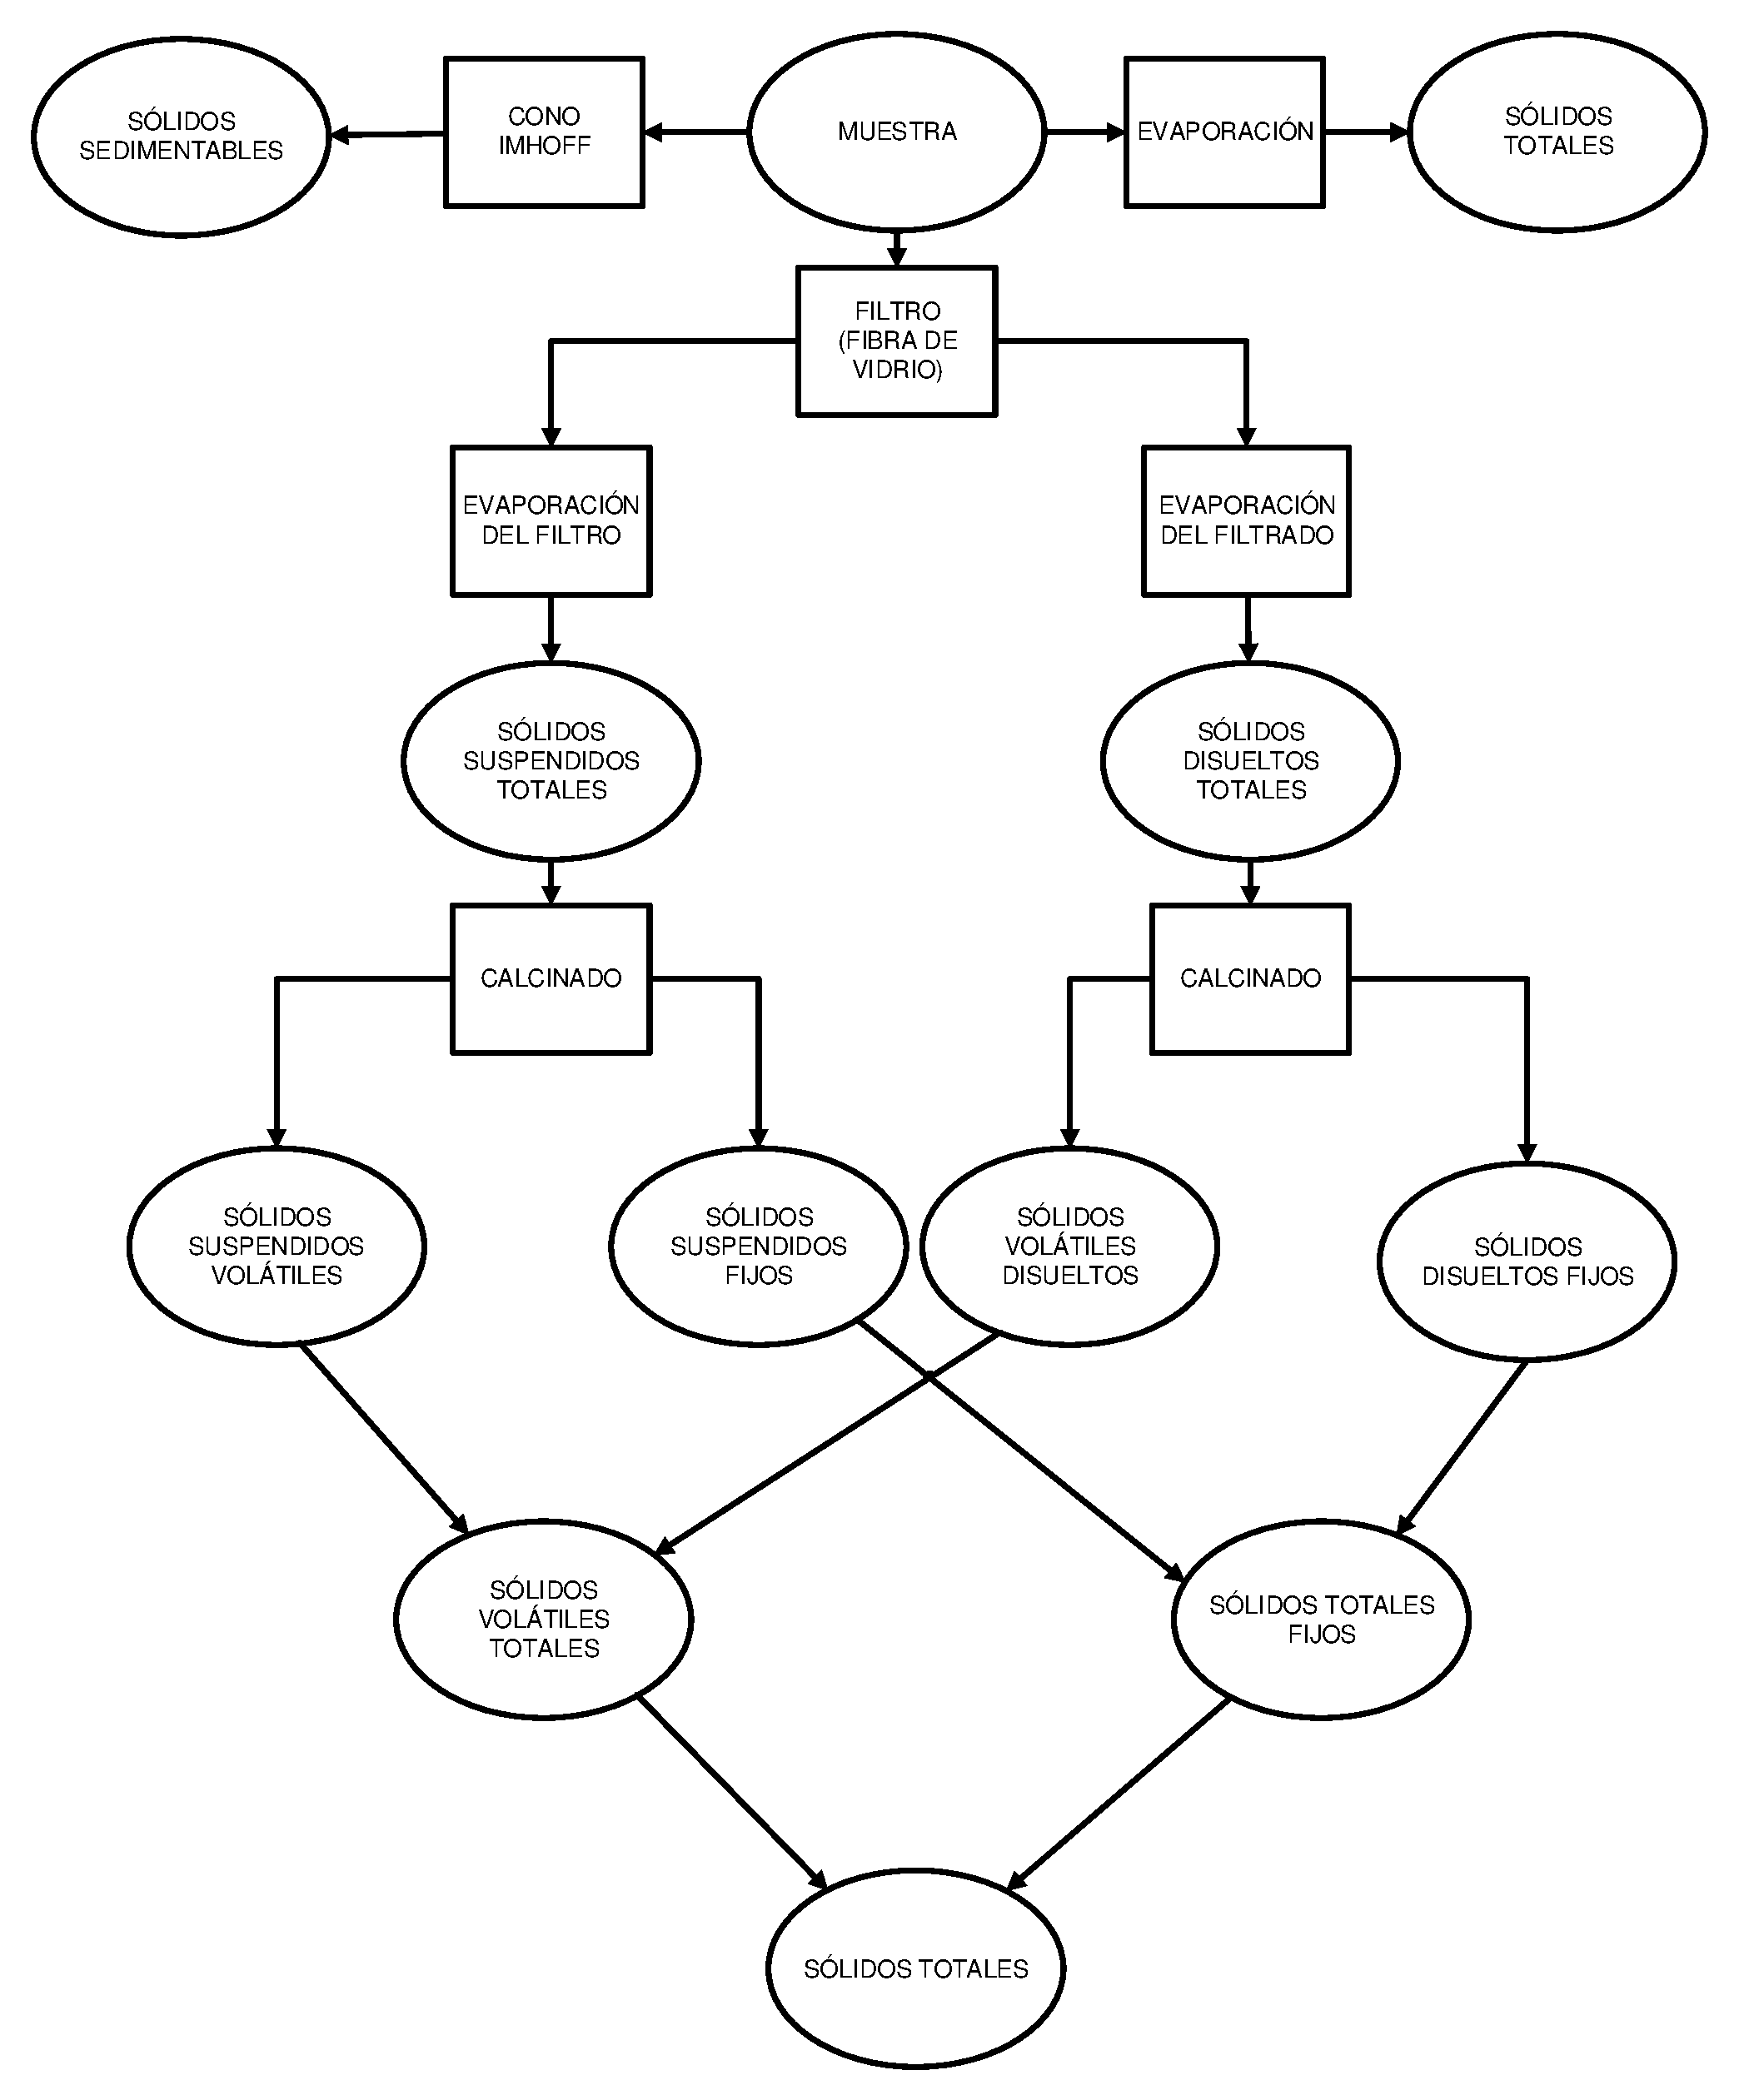
\includegraphics[scale=0.25]{../Images/Relacion_Solidos.pdf}
	\\\small{Fuente: \cite{metcalf2003}}
	\caption{Interrelación entre los tipos de sólidos presentes en las aguas residuales y los métodos de caracterización de cada uno de estos.}\label{fig:solrelcn}
\end{figure}
\begin{enumerate}[label=\textbf{$\bullet$}]
	\item \textbf{Sólidos totales (ST)}\par
	Se definen como los residuos que quedan después de que la muestra ha sido evaporada y secada a 105 °C \unichar{"00B1} 2 °C durante 24 horas en un horno de calor seco~\citep{Economia2015}\par
	Estos sólidos pueden clasificarse en dos categorías principales: sólidos suspendidos y sólidos disueltos. La suma de los sólidos suspendidos (SS) y los sólidos disueltos (SD) da como resultado los sólidos totales (ST)~\citep{metcalf2003}. La expresión matemática para los sólidos totales se puede representar de la siguiente manera:
	\begin{equation*}
		ST = SS + SD
	\end{equation*}
	Los sólidos totales son una medida importante de la calidad del agua y se utilizan en la evaluación de la carga contaminante en las aguas residuales y en la determinación de la eficiencia de los procesos de tratamiento. La cantidad y la composición de los sólidos totales pueden variar significativamente según la fuente del agua y las actividades humanas en la región.\par
	En el tratamiento de aguas residuales, el control y la eliminación de los sólidos totales son aspectos clave para asegurar la eficiencia de los procesos de clarificación y sedimentación~\citep{lazcano2016}. Además, la medición de los sólidos totales es esencial para evaluar el rendimiento de las plantas de tratamiento y garantizar que los efluentes tratados cumplan con los estándares ambientales antes de ser descargados en cuerpos receptores o reutilizados.
	\item \textbf{Sólidos Sedimentables o Disueltos(SD)} \par
	Los sólidos sedimentables (SD) son una fracción de los sólidos totales presentes en el agua que tiene la capacidad de sedimentarse en un periodo de tiempo determinado. Estos sólidos son partículas suspendidas en el agua que tienden a asentarse hacia el fondo de un recipiente bajo la influencia de la gravedad durante un período de reposo.\par
	La medición de los sólidos sedimentables generalmente se realiza mediante un equipo específico, como el cono de Imhoff o embudo de Imhoff, que permite separar y medir los sólidos sedimentables después de un periodo de sedimentación estándar, comúnmente de 30 minutos a 1 hora~\citep{metcalf2003}.\par
	\begin{figure}[H]
		\centering
		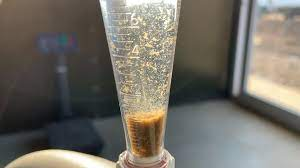
\includegraphics[scale=0.8]{../Images/cono-imhoff.jpg}
		\\\small{Fuente: \cite{aquafish}}
		\caption{Cono Imhoff, usado para determinar la sedimentabilidad de los sólidos presentes en un litro de agua residual a caracterizar en un lapso de tiempo de 60 minutos. Las unidades son expresadas en mL/L.}\label{fig:imhoff}
	\end{figure}
	La presencia de sólidos sedimentables en el agua puede indicar la presencia de partículas más grandes que pueden afectar la claridad del agua y la eficacia de los procesos de tratamiento. El control de los sólidos sedimentables es importante en el diseño y operación de plantas de tratamiento de aguas residuales, ya que su acumulación en tanques y conductos puede afectar negativamente la eficiencia del sistema.\par
	La expresión matemática para calcular los sólidos sedimentables se basa en la relación entre la cantidad de sólidos sedimentados y el volumen de agua examinado. La fórmula general es:
	\begin{equation*}
		SD = \frac{P}{V} \times 1000
	\end{equation*}
	Donde:
	\begin{itemize}
		\item $SD$ es la concentración de sólidos sedimentables en mililitros por litro (mL/L)
		\item $P$ es el volumen de los sólidos sedimentados en mililitros (mL)
		\item $V$ es el volumen total de la muestra de agua en mililitros (mL)
	\end{itemize}
	\item \textbf{Sólidos Totales Volátiles (STV)} \par
	Cantidad de materia orgánica e inorgánica que se volatiliza por efecto de la calcinación a 550 °C \unichar{"00B1} 50 °C~\citep{Economia2015}.\par
	Esta fracción incluye materia orgánica que puede ser biológicamente degradada. La medición de los sólidos totales volátiles es comúnmente utilizada en análisis de laboratorio para evaluar la cantidad de materia orgánica biodegradable presente en una muestra.\par
	La fórmula para calcular los sólidos totales volátiles es:
	\begin{equation*}
		STV = ST - SFI
	\end{equation*}
	Donde:
	\begin{itemize}
		\item $STV$ es la concentración de sólidos totales volátiles
		\item $ST$ es la concentración de sólidos totales
		\item $SFI$ es la concentración de sólidos fijos (que no son volátiles)
	\end{itemize}
	 La medición de los sólidos totales volátiles es esencial en el tratamiento de aguas residuales, ya que proporciona información sobre la cantidad de materia orgánica presente en una muestra que podría ser biológicamente tratada. Cuantificar la cantidad de este tipo de sólidos es especialmente útil para evaluar la eficacia de los procesos biológicos en una planta de tratamiento de aguas residuales, donde la descomposición de la materia orgánica es fundamental para reducir la carga contaminante del agua residual.\par
	\item \textbf{Sólidos Fijos(SFI)} \par
	Los sólidos fijos son una fracción de los sólidos totales presentes en una muestra de agua o lodo que no se vaporizan o no experimentan cambios significativos durante un proceso de calentamiento. Esta fracción incluye materia inorgánica y otras sustancias que no son volátiles a las temperaturas típicamente utilizadas en los análisis de laboratorio para medir los sólidos totales volátiles.\par
	La fórmula para calcular los sólidos fijos es:
	\begin{equation*}
		SFI = ST - STV
	\end{equation*}
	Los sólidos fijos incluyen minerales, sales inorgánicas y otras sustancias que no se evaporan durante el proceso de calentamiento. Estos sólidos proporcionan información sobre la carga inorgánica presente en la muestra y no son biodegradables a través de procesos biológicos en plantas de tratamiento de aguas residuales~\citep{martinez1999}.\par
	\item \textbf{\gls{SDT}} \par
	Es el material soluble constituido por materia orgánica e inorgánica que permanece como residuo después de evaporar y secar una muestra previamente filtrada a través de un filtro de fibra de vidrio con poro de 1.5 \unichar{"00B5}m a una temperatura de 105 °C \unichar{"00B1} 2 °C~\citep{Economia2015}.\par
	La fórmula general para calcular los sólidos disueltos totales es:
	\begin{equation*}
		SDT = \frac{P}{V} \times 1000
	\end{equation*}
	Donde:
	\begin{itemize}
		\item $SDT$ es la concentración de sólidos disueltos totales en miligramos por litro (mg/L) o partes por millón (ppm)
		\item $P$ es el peso del residuo después de la evaporación en miligramos (mg)
		\item $V$ es el volumen de la muestra de agua en litros (L)
	\end{itemize}
	Es importante destacar que la medición de los sólidos disueltos totales se realiza comúnmente en el análisis de la calidad del agua y es uno de los parámetros que se evalúan para determinar la idoneidad del agua para diferentes usos, como el consumo humano, la agricultura o la industria~\citep{martinez1999,lazcano2016}.\par
	\item \textbf{Sólidos Suspendidos Totales (SST)} \par
	Es el material constituido por los sólidos sedimentables, los sólidos  suspendidos y coloidales que son retenidos por un filtro de fibra de vidrio con poro de 1.5 \unichar{"00B5}m (ver figuras~\ref{fig:eq-filtro} y \ref{fig:filtro}) secado y llevado a masa constante a una temperatura de 105 °C \unichar{"00B1} 2 °C~\citep{Economia2015}.
	\begin{figure}[H]
		\centering
		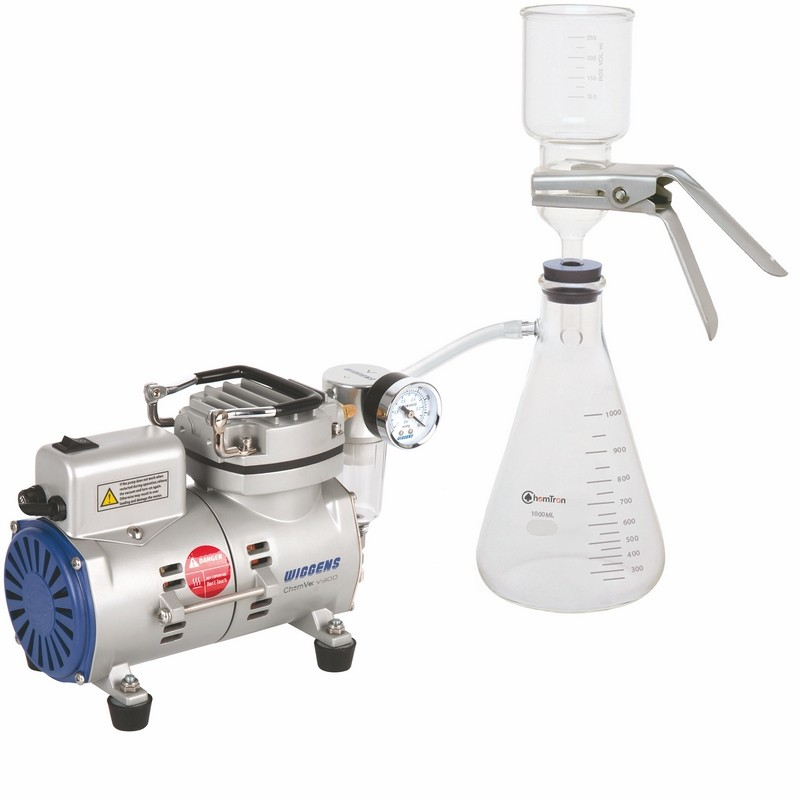
\includegraphics[scale=0.45]{../Images/filtro-solidos.jpg}
		\\\small{Fuente: \cite{Wiggens}}
		\caption{Equipo de filtración al vacío utilizado para la determinación de sólidos suspendidos totales. Su diseño permite colocar y retirar fácilmente el filtro para su pesaje y secado posterior al filtrado de la muestra de agua residual.}\label{fig:eq-filtro}
	\end{figure}
	La fórmula general para calcular los sólidos suspendidos totales es:
	\begin{equation*}
		SST = \frac{P}{V} \times 1000
	\end{equation*}
	Donde:
	\begin{itemize}
		\item $SST$ es la concentración de sólidos suspendidos totales en miligramos por litro (mg/L) o partes por millón (ppm)
		\item $P$ es el peso del residuo sólido después del secado en miligramos (mg)
		\item $V$ es el volumen de la muestra de agua en litros (L)
	\end{itemize}
	La presencia de sólidos suspendidos totales en el agua puede afectar la claridad del agua y tener implicaciones en la calidad del agua y en los procesos de tratamiento. Altas concentraciones de SST pueden causar turbidez y afectar negativamente a los organismos acuáticos al bloquear la luz y reducir la disponibilidad de oxígeno~\citep{metcalf2003}.\par
		\begin{figure}[H]
		\centering
		
\includegraphics[scale=0.4]{../Images/filtro.jpg}
		\\\small{Fuente: \cite{Lobov}}
		\caption{Filtro comercial de fibra de vidrio diseñado específicamente para la determinación de SST. Existen diferentes tipos de filtros, variando el tamaño de poro de 1.0 a 1.5 \unichar{"00B5}m, así como del material con el que son fabricados (siendo los de fibra de vidrio los más populares por su tamaño de poro y su costo).}\label{fig:filtro}
	\end{figure}
	La medición de los sólidos suspendidos totales es un parámetro comúnmente utilizado en el análisis de la calidad del agua y es esencial en la evaluación de la carga contaminante en las aguas residuales. También se utiliza en el monitoreo ambiental para evaluar el impacto de las descargas de aguas residuales en cuerpos de agua receptores y en la gestión de procesos de tratamiento de aguas residuales.\par
	\item \textbf{Sólidos Suspendidos Volátiles (SSV)} \par                
	Son aquellos sólidos suspendidos que se volatilizan en la calcinación a 550 °C \unichar{"00B1} 50 °C~\citep{Economia2015}.Los sólidos suspendidos volátiles consisten principalmente en materia orgánica que puede ser biodegradable y que se encuentra en partículas suspendidas en el agua. Esta fracción incluye compuestos orgánicos que, debido a su naturaleza, pueden evaporarse cuando se someten a un proceso de calentamiento.\par
	La fórmula general para calcular los sólidos suspendidos volátiles es similar a la de los sólidos totales volátiles, y se expresa como:
	\begin{equation*}
		SSV = \frac{P_{1}-P_{2}}{V} \times 1000
	\end{equation*}
	Donde:
	\begin{itemize}
		\item $SSV$ es la concentración de sólidos suspendidos volátiles
		\item $P_{1}$ es la peso del residuo sólido una vez secado en miligramos (mg)
		\item $P_{2}$ es el peso del residuo $P_{1}$ después de ser calcinado en miligramos (mg)
		\item $V$ es el volumen de la muestra de agua en litros (L)
	\end{itemize}
	La medición de los sólidos suspendidos volátiles es significativa en el análisis de la calidad del agua, especialmente en el contexto del tratamiento de aguas residuales. La cuantificación de esta fracción proporciona información sobre la cantidad de materia orgánica volátil presente en las partículas suspendidas, lo cual es relevante para evaluar la biodegradabilidad de los sólidos suspendidos.\par
	El control y la gestión de los sólidos suspendidos volátiles son importantes en las plantas de tratamiento de aguas residuales, ya que la eficiencia en la eliminación de esta fracción puede influir en la calidad del efluente tratado y en la carga contaminante que se descarga en los cuerpos de agua receptores~\citep{martinez1999}.\par
\end{enumerate}
\subsubsection{Temperatura}
La temperatura de las aguas residuales es un aspecto relevante al momento de realizar cualquier proceso de tratamiento (sobre todo en procesos biológicos). Puede variar según el origen de las aguas residuales, siendo comúnmente influenciada por actividades industriales. La temperatura afecta directamente los procesos biológicos de tratamiento y puede tener implicaciones en la vida acuática del receptor final~\citep{lazcano2016}.\par
La actividad biológica en el sistema de lodos activados es directamente afectada por la temperatura. Por lo general es de apreciar que a temperaturas más altas, la velocidad de reacción biológica aumenta, lo que significa que los microorganismos pueden descomponer la materia orgánica de forma más eficiente. Como consecuencia directa de tal relación, los cambios bruscos de temperatura pueden alterar la comunidad microbiana y la eficiencia del tratamiento, por lo que mantener una temperatura constante dentro del rango adecuado es crucial para garantizar la estabilidad operativa~\citep{delgadillo2005}.\par
\cite{metcalf2003} establecen como rango óptimo de temperatura para la actividad biológica de entre 25 a 35 °C ya que en rangos superiores e inferiores la actividad microbiológica se ve afectada de la siguiente manera: por encima de los 50 °C la digestión aeróbica y la desnitrificación se interrumpen, por debajo de los 15 °C las bacterias metanogénicas reducen drásticamente su actividad y alrededor de los 5 °C las bacterias autotróficas-nitrificantes entran en estado de inactividad al igual que las quimioheterotróficas, que dejan de trabajar a partir de los 2 °C hacia abajo.\par
Otro aspecto a tomar en cuenta al momento de diseñar cualquier sistema de tratamiento es que la temperatura del agua influye en la capacidad del agua para retener oxígeno disuelto, lo cual condiciona directamente la velocidad con la que los microorganismos degradan la materia orgánica (ver ecuación~\ref{eq:Hoff-Arrhenius}). A temperaturas más altas, el oxígeno disuelto tiende a disminuir, lo que puede afectar la eficiencia de los procesos aerobios en el sistema de lodos activados. Se deben tomar medidas para asegurar un adecuado suministro de oxígeno~\citep{crites2000,serway2007}.\par
\begin{equation} \label{eq:Hoff-Arrhenius}
	\begin{split}
		&\qquad\frac{d(\ln{k})}{dT} = \frac{E}{RT^2}\\
			\text{Donde:} \\
			k& = \text{constante de velocidad de reacción}\\
			T& = \text{temperatura en Kelvin}\\
			E& = \text{constante característica de la reacción en J/mol}\\
			R& = \text{constante de los gases ideales, 8.314 J/mol}
	\end{split}
\end{equation}
En general, gran parte de los autores concluyen que la temperatura óptima para el funcionamiento eficiente de un sistema de lodos activados suele estar en el rango de 20 a 30 grados Celsius. Temperaturas fuera de este rango pueden ralentizar las reacciones biológicas y afectar negativamente la calidad del efluente tratado.
\subsubsection{Color}
\cite{crites2000} advierte que el color de las aguas residuales es una característica visual que puede proporcionar indicios sobre la presencia de sustancias orgánicas, metales pesados o compuestos específicos. La evaluación del color resulta en otro aspecto importante del monitoreo de la calidad del agua y del rendimiento de los procesos de tratamiento.\par
También \cite{lazcano2016} afirma que aunque el color en sí mismo no afecta directamente la eficiencia del tratamiento, su monitoreo puede ser indicativo de varios aspectos del proceso y de la presencia de ciertos compuestos. La materia orgánica puede contribuir a la coloración del agua, y monitorear los cambios en el color puede indicar variaciones en la concentración de contaminantes orgánicos. Un aumento en la intensidad del color podría sugerir una mayor carga de materia orgánica. También es común que la formación de floculación biológica en el tratamiento de lodos activados puede afectar el color del agua.\par
\cite{Eckenfelder2000} destaca que "cambios inesperados en el color pueden ser indicativos de problemas operativos, como desequilibrios en el sistema de tratamiento". La detección temprana de estos cambios puede permitir intervenciones oportunas para corregir problemas y evitar impactos negativos en la eficiencia del tratamiento. El color del efluente tratado es un factor estético importante. Un efluente claro y con bajo color es deseable para cumplir con los estándares de calidad del agua y para garantizar que el agua tratada sea aceptable para su descarga en cuerpos receptores o su reutilización.
\subsubsection{Olor}
El olor en las aguas residuales es una característica perceptible que puede ser causada por la presencia de compuestos orgánicos volátiles y otros contaminantes. La evaluación del olor no solo tiene implicaciones en la calidad del agua, sino que también es relevante para el cumplimiento de normativas y para la aceptabilidad social en comunidades circundantes~\citep{metcalf2003}.\par
El olor desagradable, a menudo sulfuroso, puede indicar la presencia de condiciones anaerobias (sin oxígeno) en el sistema (ver figura \ref{fig:tba}). Estas condiciones pueden surgir si no hay suficiente suministro de oxígeno disuelto en el reactor de lodos activados. La falta de oxígeno puede favorecer procesos anaerobios que producen compuestos malolientes como sulfuros, compuestos nitrogenados volátiles, etc. Al monitorear los olores, se pueden identificar desviaciones en los procesos biológicos y tomar medidas correctivas, tales como: el aumento del suministro de oxígeno, la optimización del proceso de mezcla del reactor y el control del tiempo de retención hidráulico y la edad de los lodos~\citep{lazcano2016}. Además, el uso de tecnologías avanzadas, como la desodorización y la cubierta de sistemas de almacenamiento de lodos, puede ayudar a minimizar la liberación de olores desagradables.
\subsubsection{Conductividad}
La \gls{EC} del agua es la medición de la capacidad que tiene una solución para conducir una corriente eléctrica. Se encuentra fundamentada en la presencia de iones, los cuales son capaces de desprender electrones en presencia de un campo eléctrico, aumentando el valor de la corriente eléctrica cuando el valor de iones disueltos aumenta. Por lo general, el valor de EC es usado como sustituto de la concentración de SDT. Actualmente es usado como valor importante a la hora de determinar la factibilidad que tienen ciertas aguas para su uso agrícola debido a que al realizar la medición se puede determinar si existen niveles altos de salinidad en el agua usada para riego, lo cual puede afectar directamente al crecimiento de los cultivos~\citep{metcalf2003}.\par
La EC se expresa generalmente en microsiemens por centímetro (µS/cm) o milisiemens por metro (mS/m); y en micromhos por centímetro (µmho/cm)\footnote{1 mS/m equivalen a 10 µmho/cm} en el sistema estadounidense de unidades.\par
La manera mas práctica de calcular los \gls{SDT} se realiza a partir de la medición de la \gls{EC} utilizando la formula:
\begin{equation*}
	TDS \cong EC \times (0.55 - 0.70)
\end{equation*}
Donde:
\begin{itemize}
	\item $SDT$ es la concentración de \acrlong{SDT} en miligramos por litro (mg/L)
	\item $EC$ es la conductividad eléctrica de la muestra expresada en decisiemens por metro o micromhos por centímetro (dS/m o µmho/cm)
\end{itemize}
\subsection{Características Químicas}
Por regla general, los componentes químicos de las aguas residuales se dividen en orgánicos e inorgánicos. Los componentes orgánicos 
\subsubsection{Componentes Orgánicos}
\begin{enumerate}[label=\textbf{\alph*{.-}}]
	\item \textbf{Demanda bioquímica de oxígeno}\par
	
	\item \textbf{Demanda química de oxígeno}\par
	
	\item \textbf{Demanda teórica de oxígeno}\par
	
	\item \textbf{Carbono orgánico total}\par
	
	\item \textbf{Nitrificación}\par
	
\end{enumerate}
\subsubsection{Componentes Inorgánicos}
\begin{enumerate}[label=\textbf{\alph*{.-}}]
	\item \textbf{pH}\par 
	La concentración de iones Hidrógeno es un parámetro de calidad importante
	\item \textbf{Cloruros}\par 
	Los cloruros son
	\item \textbf{Alcalinidad}\par
	La alcalinidad en aguas residuales se debe a la precencia de aniones hidróxido [OH\textsuperscript{-}], carbonatos [CO\textsubscript{3}\textsuperscript{2-}], y bicarbonatos [HCO\textsubscript{3}\textsuperscript{-}] de elementos tales como lo son el calcio, magnesio, sodio, potasio y amonio.
\end{enumerate}
\subsubsection{Gases}
\begin{enumerate}[label=\textbf{\alph*{.-}}]
	\item 
\end{enumerate}
\subsection{Características Biológicas}
\subsection{Muestreo}
\subsection{Límites máximos permisibles}\label{NOM2021}
\subsection{Tratamiento de aguas residuales}
Cada año se vierten a los cuerpos de agua millones de metros cúbicos de aguas residuales, descargas municipales, industriales y agrícolas tratadas de forma inadecuada o sin tratamiento alguno.
\subsubsection{Tratamientos biológicos}
El uso de organismos vivos con el fin de reducir la cantidad de materia orgánica presente en las aguas negras se remonta a finales del siglo XIX y principios del XX en Inglaterra como resultado de varias observaciones en las denominadas \emph{granjas de aguas negras}, en donde las aguas negras provenientes de las urbanizaciones eran filtradas por medio de filtros de arena, escombros, pizarra, ladrillos, entro otros materiales pétreos porosos. Gracias a las características de estos lechos, pronto permitieron el crecimiento de varias comunidades microbianas capaces de alimentarse de la materia orgánica disuelta en las aguas residuales, reduciendo el número de contaminantes a niveles más aceptables~\citep{Fair2008}\par
A consecuencia de el desarrollo de las grandes ciudades, el uso de sistemas biológicos fue adquiriendo más usos a parte de la remoción de materia orgánica. Entre estos nuevos usos se destacan la nitrificación de aguas con alto contenido de nitrógeno amoniacal, la desnitrificación 
\subsubsection{Procesos biológicos de cultivo en suspensión}
\subsubsection{Procesos biológicos de soporte sólido}
\subsection{Lodos Activados}
Dentro de los procesos basados en cultivo de microorganismos en suspensión, uno de los más importantes, y a su vez mas utilizados, es el que involucra la utilización de lodos activados como agentes reductores de la carga orgánica presente en el afluente a tratar.
\subsubsection{Flóculos}
\subsubsection{Bulking filamentoso}
\subsection{Modelos matemáticos en el proceso de lodos activados}
\subsubsection{Modelo de Monod}
\subsubsection{Modelo de Arrhenius}
\subsection{Planta tratadora de aguas residuales municipal de Lagos de Moreno}
\begin{figure}[H]
	\centering
	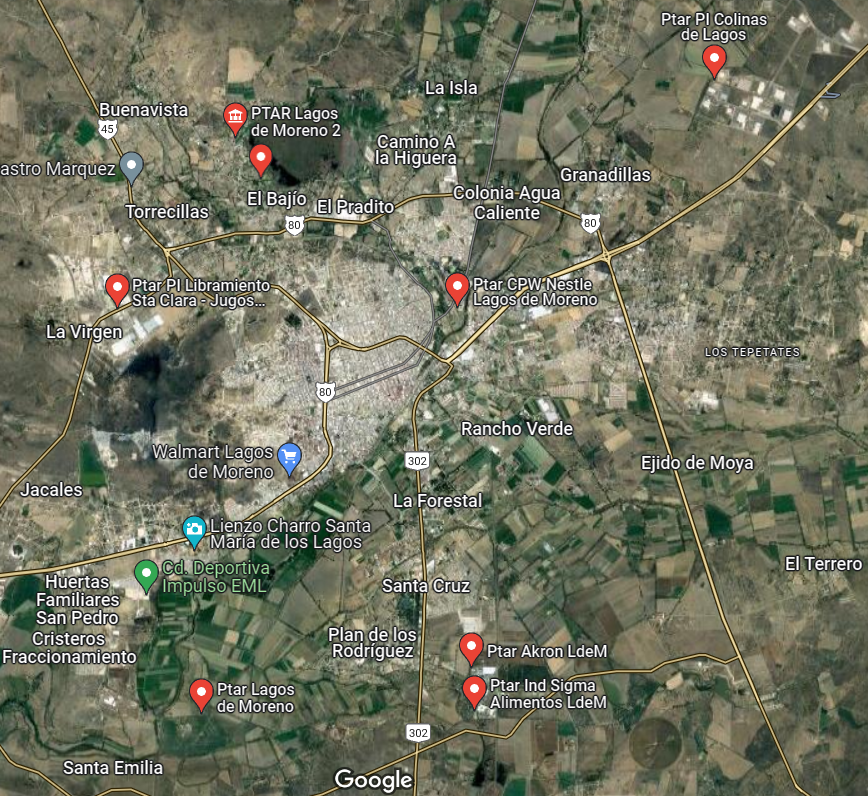
\includegraphics[scale=0.6]{../Images/PTARs_Lagos.png}
	\\\small{Fuente: \cite{Maps}}
	\caption{Mapa general de Lagos de Moreno en donde se aprecian las principales Plantas de tratamiento en funcionamiento (tanto privadas como públicas)}\label{fig:lgsptars}
\end{figure}
\begin{figure}[H]
	\centering
	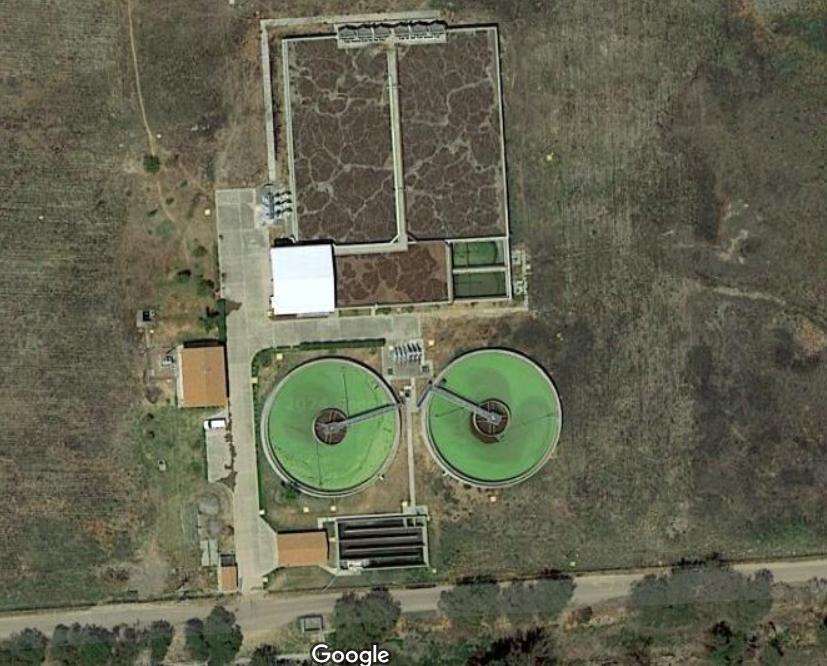
\includegraphics[scale=0.5]{../Images/PTAR_Lagos.png}
	\\\small{Fuente: \cite{Maps}}
	\caption{Imagen satelital de la planta municipal de tratamiento de aguas de Lagos de Moreno}\label{fig:lgsptar}
\end{figure}
\subsection{MATLAB®}
